\documentclass[a4paper, notoc, justified,marginals=raggedright]{tufte-book}


\usepackage[utf8]{inputenc}
\usepackage{graphicx} % allow embedded images
  \setkeys{Gin}{width=\linewidth,totalheight=\textheight,keepaspectratio}
  \graphicspath{{graphics/}} % set of paths to search for images
\usepackage{amsmath}  % extended mathematics
\usepackage{booktabs} % book-quality tables
\usepackage{units}    % non-stacked fractions and better unit spacing
\usepackage{multicol} % multiple column layout facilities
\usepackage{fancyvrb} % extended verbatim environments
  \fvset{fontsize=\normalsize}% default font size for fancy-verbatim environments
\usepackage{pgfplots}

\usepackage{lipsum}

% to see the margins and page width
% \geometry{showframe}

% Write packages versions in the log
% \listfiles


% Commands use to make the title page and page headers
\title{PhD Thesis}
\author{Clément Viguier}

% Commands use through the document


% Include documents for graphical aspects
% Color
%\input{../latex_settings/colors}
% Graph settings
\pgfplotsset{compat=newest}

\pgfplotsset{plot/.style={ 
width = \textwidth,
no markers,
color = black,
line width = 1pt,
minor x tick num = 0,
minor y tick num = 0,
        xtick pos=left,
        ytick pos=left,
        tick align=outside,
        try min ticks=2,
        max space between ticks=100pt,
  axis x line*=bottom,
  axis y line*=left,
        line join=round,
    axis line style={->}, 
        enlarge x limits=true,
        every x tick/.style={color=black, thin},
        every y tick/.style={color=black, thin},
}
}


\pgfplotsset{marginplot/.style={ 
plot,
width = \marginparwidth
}
}

\pgfplotsset{fullplot/.style={ 
plot,
width = \pagewidth
}
}

% Titles settings
%\input{../latex_settings/titles_settings}

%
%\includeonly{Introduction}

% Change the depth of section numbering and table of content to allow proper numbering
\setcounter{secnumdepth}{2}
\setcounter{tocdepth}{1}

\begin{document}


\maketitlepage

\newpage

\tableofcontents

\part*{Introduction}

\begin{fullwidth}
This chapter is dedicated to the review of literature and aims to introduce the concepts and hypotheses used and interrogated in following chapters. A link between properties of the community and the ecosystem services is first drawn, then I examine the use of functional traits to represent plants, plant functioning, and communities. Finally, the impact of intra-specific variability, in particular phenotypic plasticity, on community properties is interrogated.

While this thesis is a modelling thesis, it is not a modelling textbook, and rather than exhaustive description of the different types of models the focus will be given to selected modelling examples close to the context of this work.
\end{fullwidth}

% #######################################################################################
\chapter{Understanding community dynamics and properties: drivers and theories}\label{chapter:coexistence}

% _______________________________________________________________________________________
%\section{The different facets of plant communities: from processes to services}




% _______________________________________________________________________________________
\section{Community assembly and coexistence}

%Community assembly, drivers, interaction and dynamics.


%-----------------------------------------------------------------------------------------
\subsection{Filtering processes: from potential to realised niche}

%\paragraph{Perspectives} % What the fuck do I mean by that?

\paragraph{Plant community}

A community is defined by the ensemble of species that coexist within the same space and time intervals. Community were first viewed as group of species that have evolve together to survive within specific conditions. To maintain itself within the community, each species need to grow during the vegetative phase, survive, and reproduce. These steps of the life cycle result from the coordination of multiple physiological processes, supported by the extraction and use of essential resources: light, water and nutrients. A part of community ecology sees communities as discrete entities with specific characteristics. This view is particularly practical for management as the community type can be associated to certain properties and services, or even particular dynamics and management systems. This view is the base of phytosociology as it is still used. While a discrete approach to community ecology provide practical categorisation, it ignores the fundamental dynamic nature of living systems. In a context of global changes, considering the dynamics of plant communities is crucial to predict how these systems will react to conditions never experienced. Another approach to community ecology consider that communities emerge from the distribution of individuals of a species, distribution controlled by its genetic and physiologic characteristics and its interactions with other species (gleason 1926, whittaker 1975). The distribution of individuals depends on how it is affected by abiotic conditions and interaction with other species, or biotic conditions. The joint effects of abiotic and biotic environment are captured by the concept of niche \parencite{elton_1927}. The \textemph{niche} of a species is defined by how a species population react to abiotic and biotic conditions (resource, competition, predation, survival) and how it impact its environment. Defining the niche of a species is primarily defining the barriers that constraint the distribution of the individuals of the species.

\paragraph{Abiotic filtering}

The \textemph{abiotic filtering} designates the non biological variables that prevent the establishment of a species in a habitat. This term generally refers to climatic conditions and resource availability because temperature, water, nutrient and light availability are the main variables that constrain the plant development. Other abiotic factors can be considered, such as salinity \cite{poorter_leaf_2006} or soil properties (pH). These variables defines if a plant (depending on its specific properties) can establish a given habitat without any biotic interactions. These filters define, for a given habitat, the pool of species (or individuals if genetic variations are considered) that can grow and reproduce in this habitat without interaction. The ensemble of habitats a species can invade if only the abiotic factors are considered is called the \textemph{potential niche} (see figure \ref{fig:niche}). 

\paragraph{Dispersion filtering}

In addition to this large scale filters, another barrier may prevent a species to invade an habitat: its access. Indeed, dispersion plays a major role in the geographical extend of a distribution area of a species. Dispersion barriers such as mountains, seas or ocean prevent uniformisation of vegetation and reduction of global diversity. Such limits explain the existence of endemic species that grow only in a few locations, despite a larger potential distribution area (defined by potential niche).

%Based on genetic and physiological properties, plant species may be able to grow and reproduce in different climatic conditions.

%Potential niche

%Abiotic filtering 

\paragraph{Biotic filtering}

Finally, the main factor that can affect the ability of a plant species to establish, is living interactions. For plant species, herbivory and competition are the most important factors, but other forms of interaction can affect the potential niche. The resulting niche, after all filtering processes, is call the \textemph{realised niche}. Competition affects the growth of the focal plant indirectly by reducing the availability of resources, increasing the stress of the plant and reducing its niche (see interaction between species 1 and 3 in figure \ref{fig:niche}). Competition interactions are major factors shaping vegetation community and are extensively studied both with theoretical \parencite{chesson_general_2000, amarasekare_competitive_2003} and empirical approaches \parencite{kunstler_plant_2016}.

\begin{marginfigure}
    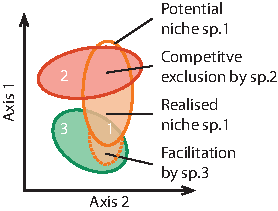
\includegraphics{./1_Introduction/graphics/niches.pdf}
  \caption[Different niches]{The potential niche of the \textcolor{myOrange}{focal} species is reduced by competition interaction with \textcolor{myRed}{species 2}, but extended by facilitation interaction with \textcolor{myGreen}{species 3}. This representation of the niche requires the knowledge of the effects of both abiotic factors and all pairwise interactions with other species. A more mechanistic approach of the niche should be considered in IMBs.}
  \label{fig:niche}
\end{marginfigure}

Similarly \textemph{facilitation} interactions also affect inderectly the levels of resources experienced by the focal plant, but in a way that is positive for the focal plant. So they widen realised niche outside the potential niche (see interaction between species 1 and 3 in figure \ref{fig:niche}). There are hypothesised to be larger along a stress gradient, where competition interactions are filtered out because they do not allow species maintenance and only positive interactions remain. Such relationships are dependent on the couple of species considered and may change depending on conditions \parencite{callaway_phenotypic_2003}.

\paragraph{Fundamental niche}
 From the point of view of the focal plant, these interactions only exist through the changes in resource availability (even if plants are able to identify their neighbours). In this sense, we can see potential and realised niches as displacements of the fundamental niche (niche defined in term experienced conditions, stresses and resources) within spaces defined by abiotic variables or biotic variables. From this framework, the fundamental niche, or conditions experienced by the focal plant, is the stronger representation of the species niche and the realised niche (abiotic and biotic filters on the niche) emerge from the effects of external factors on this experienced environment.

This point of view should be adopted in models \parencite{berger_competition_2008} because it allows the representation of both abiotic and biotic factors in a shared and generic framework. This is an improvement in comparison to model requiring matrix of interaction coefficient between species. Such matrix, in addition to be hard to parametrise, cannot be used in a framework of dynamic strategies. Modelling effort should instead be on explicit temporal and spatial dynamics of resource dynamics. Plant interactions would be captures by the effects of plant functioning (reduction of resource levels in relation to plant growth and resource use) on these dynamics \parencite{berger_competition_2008, morin_comparing_2009}.
%Biotic filtering - realised niche.

%Abiotic drivers main tnhing at global scale... Then interactions and competition.

\textbf{The concept of ecological niche serves as a great tool for theoretical research on coexistence. It encompasses in a convenient way both abiotic and biotic filters of one species distribution. While traditional view of the niche require to consider both abiotic filters and pairwise interaction, fundamental niches and resource dynamics modelling offer an alternative to model realised niche as an emergent property of the model.}


%-----------------------------------------------------------------------------------------
\subsection{The complexity of coexistence}

\paragraph{The question of coexistence}
If ones want to better understand and predict dynamics of complex systems, they first need to understand how such complex is assembled. Niches can be used to characterised a range of habitats a plant can live in, but because of complex inter-specific interactions, determining the final composition of a community from the list of species that can live in this habitat is not easy. If it is easy to observe diverse ecosystems (from bacteria, to plants, insects or algea), it is challenging to determine the processes that 1) group the entities together (in time and space), 2) maintain an apparent stability in the group composition (at least at a certain spatial and temporal scale). 
We can image imagine biotic filtering as an physical filter, the same way abiotic filter is often illustrated, but this image does not translate the dynamic and complex nature of underlying processes. Biotic filtering emerge as the result of all the interactions between the entities that make it through the other filters. And how these interactions, direct or indirect, play together determines the stability of the diversity.\\

To predict the outcome of competition interactions multiple theories have been developed. Among these theories, we can cite two that have different perspective on the same question: how do species whering resources coexist in an homogeneous environment?

\cite{chesson_mechanisms_2000} tends to have a population dynamic view of the system and identifies two types of processes that promote coexistence: (1) stabilizing mechanisms, (2) equalizing mechanisms. The former are required to stable coexistence as it a condition of invasibility. In other words, plants can coexist only if one species can invade the other. The condition to such invasion is that the species at low density growth better that the species at high density. This is the case if intra-specific competition is higher than inter-specific competition. Equalizing mechanisms are processes that diminish the fitness differences between the species, without ensuring stable coexitence. This framework is extended by \cite{adler_niche_2007} in the modern coexistence theory. It states that niche differences and fitness differences are the two mains axis of species coexistence. They make the assumption that niche differences define the relative strength of inter-specific versus intra-specific competition. The larger the differences between niches, the thiner is the overlap, and the weaker the inter-specific interactions. Therefore, this can be related to stabilizing mechanisms in \cite{chesson_general_2000}. On the other end, fitness differences also impact coexistence. The lower the differences, larger are the chances species coexist. The importance of niche differences required for stable coexistence decrease with the decrease in fitness differences.

In the other hand, Tilman elaborates a theory \cite{tilman_resource_1982, tilman_plant_1988} around resource use more in line with the idea of fundamental niche expressed in previous paragraph, the contemporary niche theory. Species are characterised by the impact they have on the resource, and they use the resource for growth. Competition is in favour of the species with the lowest requirement for the resource because competition leads to resource deprivation it can survive. But coexistence if there is more than one limiting resource. In this case, coexistence can be achieve if species have a stronger impact on the resource from which they benefit the most (and intersecting zero net growth isoclines). 


These two theories give strong conditions for stable coexistence, however they required simplifying hypotheses (all other things being equal, homogeneous environment) that are not met in natural environments. Despite their different appraoches, these theories can be united as demonstrated by  \cite{letten_linking_2017} if the impact and benefit coefficients from contemporary niche theory are transltaed into niche and fitness differences. Despite this unified theory, they applied to a too limited range of situation to be applicable in the context of diverse mountain grasslands.
%
%
%
%Focus on interaction: chesson modern coexistence theory.\\
%
%Chesson vs Tilman. 
%Chesson focuses on interaction and 2 by species, give central idea of stabilizing vs fitness difference.\\
%Tilman focuses more on resources, how the use and impact on resources affect competition and can enable conexistence, but limited coexistence according to this criterion: plankton paradox. No heterogeneity, no temporal dynamics\\
%
%Other things being equal hypothesis (in models at least) does not allow the full diversity to emerge.\


%Plankton paradox in homogeneous system, where abiotic and dispersion should have little role into maintenance of species diversity.\\


%\textbf{One mechanisms alone seems to not be enough to explain fantastic diversity observed in natural ecosystems. However there are multiple theoretical mechanisms that support species diversity and that should taken into account in community models: diversity of resources, spatial and temporal variability, frequency dependent effects, etc...}


\textbf{Plant community require strong coexistence mechanisms to maintain species richness. Single theories fail to predict high diversity observed in plant communities such as natural mountain grasslands. However, high dimension coexistence processes and complexity seems to be an answer to the biodiversity paradox. In addition to niche based coexistence processes, other mechanisms that promote coexistence must be considered.}




% _______________________________________________________________________________________
 \subsection{Variability and dynamics: driven by the resource}


%-----------------------------------------------------------------------------------------
%\subsection{The complexity of community dynamics} % not very informative title%

Resource dynamics, even with constant influx, seems to be the key of understanding plant interactions and dynamics according to Tilman \cite{tilman_plant_1988}. Can the resource distribution is time and space explain coexistence?

\paragraph{Community dynamics}

In Tilman's perspective, resources are driven by two things, external influx and internal (to the system) consumption or cycle. The system strucutre and composition is responsible for resource dynamics as much as external influx. And these dynamics alter the structure of the community and change the hierarchy within the community. This cycle is well illustrated by the cycles we can observe in forest systems and gaps models. Mature forests produce big trees that fall down and create perturbation within the system. The resulting hole in the canopy allows for pioneer species to invade this space without competition. While they grow, other slower species are in shadows and must tolerate this competition, and grow enough to out-compete first established species. Because there is trade-of between potential growth and shade tolerance allowing this cycle to set up, there is a succession dynamic after each perturbation of the systems. These local events of perturbation support coexistence as a large scale, coexistence that can be captured by spatially explicit models \cite{chave_study_1999, falster_plant:_2016}.

\paragraph{Temporal heterogeneity}

\begin{marginfigure}
    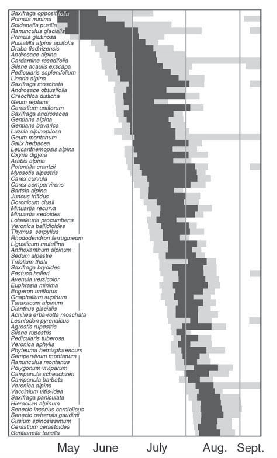
\includegraphics{./1_Introduction/graphics/flowering_m.pdf}
  \caption[Flowering periods of alpine species]{Diversity of flowering periods of alpine species. Evidence of succession in grassland ecosystems. From \cite{korner_alpine_2003}.}
  \label{fig:flowering}
\end{marginfigure}

Such drastic dynamics do not exist in mountain grasslands communities. But the natural temporal variability of resources due to contrasted seasons, also drives diversity in growth strategies. Coexistence comes the existence of multiple climatic contexts at the same place (but not the same time). As plants cannot be the most competitive species for any given condition in the whole range of conditions experienced in mountain habitats, there is a succession of species at the top of competition hierarchy \parencite{adler_climate_2006} (see figure \ref{fig:storage_effect} for illustration). The diversity of flowering periods in figure \ref{fig:flowering} is an evidence of this succession dynamics.

\begin{figure}%[tb]
    \classiccaptionstyle
\sidebysidecaption{0.60\textwidth}{0.3\textwidth}{%
    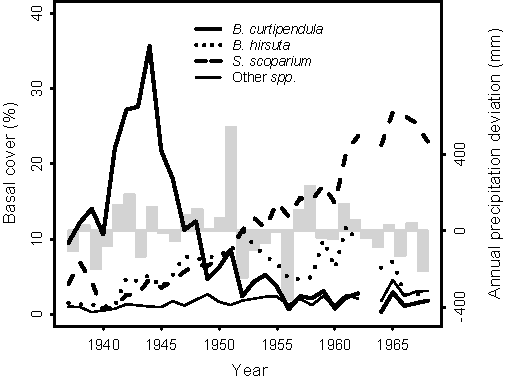
\includegraphics[width=1\linewidth]{./1_Introduction/graphics/succession.pdf}%
}{%
  \caption[Changes in dominance for 3 grassland species]{Changes in observed basal cover for 3 grassland species. This variation in hierarchy illustrate the succession in grassland communities and the storage effect due to the stabilizing effect of climatic variation promoting coexistence. See details in original study by \cite{adler_climate_2006}.}
  \label{fig:storage_effect}
  }
\end{figure}

This mechanism promoting coexistence because of succession dominance driven by temporal changes in environmental condition is called storage effect. The species grow when the conditions match their niche, and store the gains to wait until next favourable conditions. This term is generally applied to yearly variations, but the idea can be applied for variations within a growing season, allowing growth and storage until next season.

%
%from tilman: dynamics of resources
%
%gap model, succession in forest
%
%less structure in grasslands, but also diversity between early and late 
%
%
%
% Succession coexistence and forest models. Dynamics of resources, influx versus impact. Storage effects. Heterogeneity. But how does it link to traits.

%\textbf{From the multiple first attends to explain coexistence with one particular mechanism, scientific community realised that indeed multiple mechanisms are at work to make species diversity in ecological community. 
%multiple drivers that filter down. + temporal effect (metacommunity, invasion, equilibrium vs long transitions)
 % This multiplicity highlight the need for unifying framework able to cover this diversity of mechanisms and dimensions.}
 
 
\paragraph{Spatial heterogeneity}

The temporal variations have a stabilizing effect on coexistence \cite{tilman_plant_1984}, but maybe more intuitively, spatial heterogeneity also promotes coexistence. Indeed, spatial variations of conditions at small scale create multiple niches that allows for diversity if measured at higher scale. This spatial heterogeneity can be overlooked, but in the context of mountain grasslands where plants are generally small due to high stress levels and very fine scale heterogeneity due to terrain texture it can play as a strong stabilizing mechanism.

%
%tilman 1982, spatial
%chesson, 1994, temp, 
%storage effect admer 2006
%even if stochasticity can reduce coexistence. Fine scale heterogeneity is rarely taken into account, but can play an important role, especially with small individuals.

\textbf{Spatial and temporal heterogeneity play a major role in coexistence maintenance by creating various opportunity, or niches, in a given ecosystem. Internal dynamic variation of conditions also support stable coexistence.}

\subsection{The complexity of diversity}

\paragraph{Larger scales dynamics}

While resource use strategies and resource heterogeneity are important mechanisms for diversity, dispersal processes and meta-community dynamics should also be considered.

Role of meta community and dispersion dynamcis, network effects

\paragraph{Embrace complexity}

\parencite{clark_resolving_2007}: coexistence is highly dimensional


 
 % conclusion of the section/chapter:
 \textbf{The evaluation of services relies on a good representation of the plant community and its essential properties. To represent complex interacting systems like vegetation communities, descriptive approaches are not sufficient and driving processes must be considered. Explicit heterogeneity and dynamics of the resources is key to understand and model filtering processes, coexistence mechanisms and community dynamics. Modelling both community properties and resource dynamics require understanding of plant functioning and diverse growth strategies.}
 
 
% #######################################################################################
%\chapter{Considering strategies and functional traits}

\chapter{How to represent plant community}

All plants share the same pool of essential resources and similar physiological processes of assimilation and allocation, however species differ by their growth rates and niches. How such difference emerge  from common functioning framework? Species differ on parameters that characterise this functioning. The challenge of modern community ecology is to determine the trajectories existing ecosystem will follow under new environmental conditions. Species centred approaches, because they are limited to the knowledge of existing response patterns to existing gradients, cannot tackle this 
problem. How can changes of the representation of plant allow generalisation of plant functioning to new conditions?
%Same resources: even more difficult to understand coexistence. Must have differences on how they gather and use these resources. Species is not a handy tool to describe differences in functioning and strategies. Shift in paradigm needed.

% _______________________________________________________________________________________
\section{The continuity of functional ecology}

\subsection{Shift in paradigm: traits and patterns}
 blabla bla 

Measure of respiration, assimilation : better insight on the differences between species. Better understanding of plant functioning. Also show that there is a continum in plant functioning. This continuum is in line with the observed continum of community.

\paragraph{A shift needed}

Classical use of niche theory can be observed in Species Distribution Models (SDMs) that link the probability of presence of one species to multidimensional description of an habitat. The environmental variables are literally used as the dimensions of the Hutchinsonian niche, and directly link the species to its fitness in a given environment (see figure \ref{fig:paradigm_shift}, first row). This method is widely used to model environmental niche, but some can also include species interactions to incorporate explicitly biotic filter. SMDs have good theoretical support and have a lot of practical applications, however their strength is reduced at the scale of the community where the biotic filtering processes and fine scales dynamics take the advantage over large scale abiotic filtering. Also, because they require a lot of data for any given species, they lack generalisation properties to be applied to rich communities. Community dynamics require fine scale plant functioning processes to capture the effects of small scales variability and plant interactions, drivers of coexistence. 

This example of modelling approach based on a species centred framework reveals the weaknesses of this framework. The distribution of a species along gradients, or its niche, while it can be capture by abiotic variables, is primarly determined by the fitness components (and wheather or not they lead to a positive fitness): growth, survival, reproduction. These variables are not intrinsic properties of species, but emerge from the interaction between physiological processes (carbon assimilation by photsynthesis, water absorption, organic matter allocation, etc...) and the environmental conditions. Only considering these processes allow to explicit and decompose plant functioning, and therefore model it in new combinations of environmental conditions.

\begin{figure}
    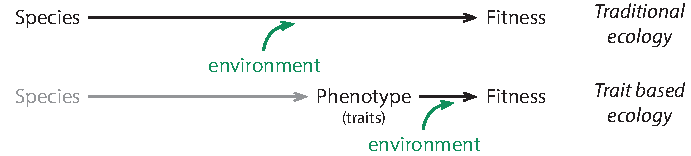
\includegraphics[width=1\linewidth]{./2_PP/Figures/Concepts/species_to_fitness.pdf}
  \caption[From discrete to continuous link between species and fitness]{The shift toward trait based ecology allows for the decomposition of the link between species and fitness determined by the environment. On one hand, the link between species and traits is better characterised by standardised protocols and the use of databases such as TRY \parencite{TRY}. On the other hand, the link between phenotypes (defined by trait values) and fitness can be generalised and the role of environment on this relationship better understood.}
  \label{fig:paradigm_shift}
\end{figure}

Most of plant species share the same growth, survival and reproduction processes, but they still differ in these aspect as a function of the abiotic and biotic environment. The solution to shift from species centred paradigm, and its couple habitats-species (or species-environment-abundance like in SDMs), is to explicit the phenotype of these species. By using functional traits to define the phenotype of a species, ecologist can limit the representation effort to the link between traits and fitness physiological properties \parencite{reich_leaf_1992}, and then link species to traits with simpler data collection procedure \parencite{cornelissen_handbook_2003} (see figure \ref{fig:paradigm_shift}, second row).


This shift in paradigm allows for a simpler and functional representation of plant species, that can be latter link to physiological or ecological processes.

%diaz, lavorel, glopnet and try

%this shift worked: falster, 


\paragraph{The rise of functional traits}

The functional traits allows to decompose the link between species and fitness, but requires an extra step as two links must be defined. 

Collection of multiple trait sampling.

\paragraph{Traits and gradients}


change of traits along gradients. Is it interesting?



\textbf{The complexity of coexistence and community dynamics processes could not be captured with traditional species centred ecology. The last two decades saw the rise of functional ecology and its ability to capture quantitatively relationship between vegetation and abiotic gradients. The capacity to }

\subsection{Understanding interaction and competition: a question of symmetry?}

Functional traits can be used to determine the response of species or communities to an abiotic factors, or link morphological traits to physiology. It is also argued that they can capture responses to biotic factors. Traits could be used to 

CAUTION: do not mistake symmetry of competition (function of delta tratis) with form of competition (georges presentation). 


niches and gradient - symetric vs hierarchical 

symetric an assymetric interaction: it could change the interpretation: identify which traits are in what case.


\parencite{kraft_functional_2008}
often need to use multiple traits \parencite{kraft_plant_2015}


traits used as a proxy for plant interaction and competition. /!\ can be context dependent \parencite{gallaway_2003}.

but non transitivity: key role in maintenance diversity \cite{levine_beyond_2017}.

\textbf{Traits are good proxy for competitive interaction and fitness differences. .. a bit more complex. If the interaction is transitive, a strong asymmetric pattern can be observed between interaction effects and trait differences, while symmetric interaction reveal niche differentiation processes. Despite these observed relationship, alternative mechanistic solutions must be adopted to capture the multi-dimensional and context-dependent nature of plant interactions.}


\textbf{The paradigm shift toward functional ecology allowed the shift from discrete to continuous representation of species. This change makes easier the representation and study of plant communities, especially along conditions or management gradient. Traits are also used to study plant interactions.  Trait approaches offer a functional link between morphology and physiology that has great potential in generalising environmental effect on phenotype-fitness relationship. However, the need for multiple traits to capture plant niche differences or similar response patterns of multiple traits suggest underlying structure within trait assemblage. Understanding this structure and how it relates to community dynamics external drivers is crucial in the representation of diverse communities. } 

%Despite the advantages of functional traits, close comparisons and links with theoretical approaches should be used carefully, and underlying assumptions should be interrogated.




% _______________________________________________________________________________________
\section{How trade-offs make strategy space}

%-----------------------------------------------------------------------------------------
\subsection{Trade-offs: capture constraints on species differences}

\paragraph{Leaf Economic Spectrum}
The functional link that is observed between some morphological traits and physiological traits suggests underlying processes that link these traits together. It appears that multiple traits are correlated together at the global scale between species \parencite{reich_evolution_2003,	 wright_worldwide_2004, chave_towards_2009, reich_world-wide_2014} and within species \parencite{hu_novel_2015}. This coorelation between functional traits of the leaf was described at a global scale by \cite{wright_worldwide_2004}. The \textemph{Leaf Economic Spectrum} (LES), defined by these correlations between multiple traits, draws a continuum of strategies. It spreads from species with high resource acquisition rates and rapid growth rates but low tissue lifespan, to species with longer tissue lifespan but lower growth rates. This is a clear description of a \textemph{trade-off} between strategies, opposing exploitative strategies (high Specific Leaf Area (SLA), high Leaf Nitrogen Content (LNC) and low Leaf LifeSpan (LLS)) to conservative strategies.


\begin{marginfigure}
    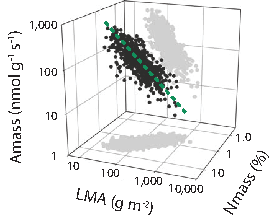
\includegraphics{./Figures/LES1_m.pdf}
  \caption[Leaf Economic Spectrum]{Three dimensions of the LES. Correlation of Leaf Mass Area, assimilation rate per mass unit and nitrogen concentration. This correlation reduces three dimensions (more dimensions not shown) into one axis (\textcolor{myGreen}{- -}).}
  \label{fg:insurance}
\end{marginfigure}

This axis of differentiation allows ecologist to link quantitative measures to types of strategies that better capture diversity of strategies than discrete typology. These strategies are translated in traits, traits that can be translated into physiological processes parameters, then into components of fitness.

In addition to a quantitative measure of species strategies, such trade-offs simplify a lot trait-based approaches. While many variables can be measured on one individual, correlations between these variables reduce the number of dimensions to considered. This simplification cannot be better illustrated by the work of \cite{diaz_plant_2004} that demonstrate the existence of two major axis of "evolutionary specialisation" that explain most (41\%) of trait variability: siez related traits, and resource use speed traits. Similar evidence is also found at global scale in addition to evidence for high levels of coordination between axis \parencite{diaz_global_2016}.


Similar correlations could be found in roots \cite{ ryser_importance_1996, reich_world-wide_2014}

Where does it come from : shipley : morhpological constraints (as for seed size and seedling growth and survival), hard frontier plus soft frontier (small figure).

Diversity of mech: diveristy of strategies. more or less independent.\\

\textbf{Trait-based ecology rapidly lead to the observation of trait correlations and trait syndromes between plants. These axes of differentiation emerge from processes that constraint plant strategies. Better characterisation of these constraint should allow a better representation of plant functional diversity.}

%-----------------------------------------------------------------------------------------
\subsection{Strategy-spaces made of trade-offs}

Global functional trait dataset and databases revealed global scale correlations between traits. These correlations, or trade-offs, simplify the representation of plant species \parencite{diaz_global_2016} and translate fundamental axis of strategy differentiation \parencite{reich_world-wilde_2013}. Yet, plant community exhibit extraordinary species and functional diversity suggesting that not all traits are correlated. Trade-offs emerge because of hard (physical, chemical or biological) and soft (competitive pressure) constraints on combinations of functional traits. Therefore, for a given couple of traits, the physical independence of traits and the independence of ecological processes they are involved in should insure the absence of trade-offs between those. While some traits are related to multiple physiological processes (a composite traits like SLA is involved in water regulation, but also light capture), traits are often specific to a processes...
Same number of strategy axis than filtering processes. (avoidance vs resistance, drougth, frost, but could be applied to competition for resources )


reich, wright, shipley, diaz.

\paragraph{Empirical evidence}

support of CSR triangle \cite{frenette-dussault_functional_2012, pierce_allocating_2013}

\textbf{The multiplicity of processes shaping vegetation systems leads to similar constrained diversity in plant strategies. These strategies are captured in a strategy space drawn by independent trade-offs tightly related to functional traits. These functional trade-offs have great potential in the representation of a functioning plant diversity, while parameter set allows easy characeterisation of species and communities.}



% _______________________________________________________________________________________
\section{How traits link to ecosystem properties}

The link between community properties and ecosystem services has been mentioned in chapter \ref{part:introduction}, this section develops processes involved and how functional traits are integrated into this link.

%-----------------------------------------------------------------------------------------
\subsection{Mass Ratio Hypothesis, Community Weighted Means, and functional identity}

As explained, plant species, based on their identity, provide ecosystem services. Some of these services are direct consequences of the characteristic of the species and their functioning. The greater the abundance of a species that supply particular ...

Because functional traits are quantitative variables, they can be manipulated more easily than factors. Therefore, while phytosociology describe vegetation communities with broad types and approximate abundances, trait-based ecology benefit from this continuity to characterise mean properties of community. The \textemph{Community Weighted Mean} of a functional trait is the average of species specific trait values weighted by the relative abundance of each species, and correspond to a mathematical application of the mass ratio hypothesis. These summary variables define the communities in a quantitative way similar as functional trait for species. In addition to be quantitative, it is functional and responses to disturbing factors can be predicted \parencite{lavorel_predicting_2002}.


grime1998, shipley 2006
\textbf{According to the Mass Ratio Hypothesis, some properties of the community directly scale to the characteristics of the most abundant species. In this hypothesis, the \textemph{functional identity}, defined by functional trait values, has more importance than the identity of the species. Community Weighted Mean measures generalise this hypothesis using mean species trait values. While these tools can link community composition to ecosystem properties and services, they require precise measures of plant functional traits to be reliable.}

%-----------------------------------------------------------------------------------------
\subsection{Benefits of diversity}

Certain processes are determined by the most abundant species of a community, but other services and functions may result from the properties of the group. Diversity is the most important property of an ecosystem or a community for wide audience. This measure is peculiar to groups of organisms and plays a major role in its functioning and the services it provides. Diversity can refer to species richness or functional diversity. The former quantifies the number of species present in a habitat and can take into account the relative abundance of the species. Many indexes can be used to measure this variable representing different perspective or aspect of the metrics (see \cite{chalmandrier_communities_2015} for exhaustive information).

Empirical studies demonstrate the importance of diversity for multi-dimensional services ... Services are: ......

Diversity also supports functions and other properties of the system. Multiple mechanisms explain this multiplicity contained in the measure of diversity. 


\begin{marginfigure}
    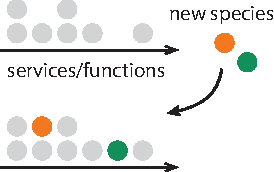
\includegraphics{./Figures/insurance_m.pdf}
  \caption[Diversity insurance effect]{Insurance and selection effects. New species increasing diversity either reinforce existing function (\textcolor{myOrange}{$\bullet$}), or provide new function (\textcolor{myGreen}{$\bullet$})}
  \label{fig:insurance}
\end{marginfigure}


First importance of species richness in found in the insurance effect that prevent the loss of a function or a service with the loss of a species by insuring that multiple species provide such function or service. Another way of seeing this notion is the selection effect that states that increasing diversity increases the potential number of services provided by the community, as each species added can provide new function/service (or at worst reinforce already present ones). This second concept is at the edge of the insurance effect

benefit of species diversity: insurance effect - portfolio effect ?

selection, niche complementarity

what about functional convergence

productivity 

\textbf{}

\subsection{Productivity: both community property and ecosystem services}

Productivity of a plant community is mostly sensitive to abiotic conditions (precipitation and temperature). 
Productivity as a marker of abiotic conditions and 

Productivity as a property: depends on the community structure and properties. Leads different services.

Productivity as a service itself: production (fodder in this case, but OM in forests).

\textbf{}

%-----------------------------------------------------------------------------------------
\subsection{Trade-offs in ecosystem properties}

lavorel 2012 : trade-off  \parencite{lavorel_how_2012}
traits - related to trade-off in ES bundles, mostly driven by climate change (rather than management) \parencite{lamarque_plant_2014} limits ?
%\textbf{}


% Section/chapter conclusion
\textbf{The shift from species centred paradigm to trait approaches unlocked numerous discoveries in plant community ecology. In addition to facilitate the study of the effect of abiotic conditions and biotic interaction, traits can be used to describe the community and its main properties to evaluate ecosystem services.}

%\textbf{However, the accumulation of trait measurements useful for the study of gradient response patterns and community structure, also reveals the variable nature of traits.}



% _______________________________________________________________________________________
\section{Modelling diverse plant community}

Modelling mainly consist in deciding what is important considering and worth representing. The choice of how an entity or a mechanisms is represented also correspond this decision making. While considering vegetation community the choice can be on the resources needed, the type of perturbation, or the part of the life cycle of most importance. For vegetation models for the study of community properties and dynamics, the representation of the interactions of multiple species is key. Strategy space concepts offers a great solution to both the interactions and the diversity of species, while also informing the modellers of the communities' properties.

%-----------------------------------------------------------------------------------------
\subsection{How strategy space open vegetation modelling}

%In a mechanistic model with multiple species, strategy space are simplified ways to define multiple species. Species identity is fully defined by its position in this space of species specific parameters.

\paragraph{Theory to traits}

Plant diversity is expressed and in visible to anyone by the variation in shapes and colors, scents and growth forms, but this diversity is the demonstration of the multiplicity of strategies. In a early attempt to make sense of this diversity of strategy \cite{grime_evidence_1977} theorise the existence of two type of constraints that shape plant communities: perturbations and stress. The perturbation axis captures the variability of community drivers, while the stress axis captures how conditions facilitate or make difficult plant establishment. They draw a two-dimensional space where three regions can be invaded\sidenote{high stress and high perturbation regions does not allow establishment}, corresponding to three different strategies: competitive (C) in low stress-low perturbations region, stress tolerant (S) in high stress-low perturbations region, ruderal (R) in low stress-high perturbations region, forming Grime's triangle (\see figure \ref{fig:grime_triangle}).

\begin{marginfigure}
    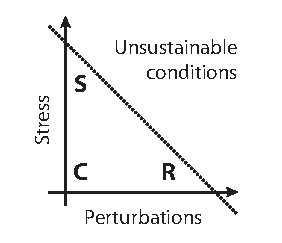
\includegraphics{./Figures/Grime_triangle.pdf}
  \caption[Diversity insurance effect]{Grime's triangle. Competitive (C), stress tolerant (S), and ruderale (R) strategies are dominant in the three regions of the perturbations-stress space.}
  \label{fig:grime_triangle}
\end{marginfigure}

Grime's triangle set the basis for strategy space, and the broad meaning of \textit{stress} and \textit{perturbations} terms allow them to be applied to various conditions. However, the diversity of types of stresses (drought, cold, nutrient availability) and perturbations (predation, fire, avalanches etc...) cannot be specificaly captured by such wide concepts. \cite{westoby_leaf-height-seed_1998} highlight the difficulty to use such space and its incapacity to explain some patterns. According to him, a strategy space\sidenote{called Plant Ecology Strategy Scheme (PESS) in his paper} should: 
\begin{itemize}
\item "express meaningful differences in ecological behaviour between species";
\item allows to "position a plant species from anywhere in the world within";
\item be composed of attributes that "require little enough effort to estimate";
\item lets "possible to quantify the extent to which the [strategy-space] captures variation in other plant attributes".
\end{itemize}
He proposes to use functional traits to meet these criteria of functional differences, generalisation, and practicality. Three traits capture the components of Grime's triangle:
\begin{itemize}
\item Specific Leaf Area (denoted L): captures the speed of return of investment of carbon in leaf, as latter highlighted in the LES. High SLA is generally associated to competitive species that capture a lot of light and have a high growth rate. At the other end of the spectrum, low SLA species are more stress tolerant. This axis is the practical equivalent to hte axis CS in GRime's triangle.
\item Height at maturity(H): race to the light (but not time fixed as protocol for functional trait encouraged it), but also capture ruderal axis (time interval between perturbations)
\item Seed mass (S): expresses the capacity of a species to invade freshly disturbed environments or the competitive advantage seedlings possess with a larger starting carbon pool. This trade-off between competitive strength of seedlings against chance of invading freshly disturbed environment capture well the CR axis of Grime's triangle.
\end{itemize}
The LHS strategy space proposed by Westoby has the advantage 


\paragraph{In DGVMs}

Strategy space proposed by Westoby 

Dynamics Global Vegetation Models tend to use such strategy spaces to model high diversity with limited number of traits. 

Simplification: limited number of straits: DVGMs

translate traits into physiology: easy

diversity of strategies

specific trade-off related to the context \parencite{scheiter_impacts_2009}

\paragraph{In IBMs}

why not too much on IBMs (but Reineking, Marechaud ?, falster, meh, I guess that Lohier's and Maire's are sort of strategy space) - because lower community models at this scale: gap to fill.

But when it's used: break the growth function that links phenotype, genotype and environment ( see figure \ref{fig:paradigm_shift}). Same growth function: no need for specific parameters: smae rules for all, but different phenotypes. (the concept of genotype and phenoptype would merge for functional traits, if there was not other control on other aspects, phenotype defines itself). This is important as it allows for intra-specific variations that would necessite more complex function in the first paradigm. 

The growth function, in a simulation model includes all steps from resource gathering and transformation, biomass allocation and phenotype alteration (\textit{e.g.} frost, graing \textit{etc}...), takes as inputs the phenotype and environment, and gives the new state of the phenotype (and environment). 

 figure \ref{fig:paradigm_shift}

This last paragraph is important to link with the plasticity in a later paragraph.


%-----------------------------------------------------------------------------------------
\subsection{How models inform us on properties and dynamics}

\textbf{The use of strategy spaces in models allows the representation of high diversity in a common plant functioning framework requiring limited number of parameters. Such approaches are very useful to follow the dynamics of communities in a mechanistic framework. Individual models tends to ignore such simplifications procedure and relies on direct measure of traits of interest because they generally integrate a limited number of species. IBMS can take advantage of trade-offs and simple strategy spaces to model diverse communities at small scales while keeping biological mechanisms at their core. However, model based of strategy space tend to consider mean individuals and ignore the individual variations.}


% #######################################################################################
\chapter{The importance of phenotypic plasticity as a specific case intra-specific variability}

% _______________________________________________________________________________________
\section{Intra-specific variability change the rules}


%-----------------------------------------------------------------------------------------
\subsection{Increasing interest in intra-specific variations}

Trait approaches emergences lead to a better understanding of general patterns of community responses to drivers and of trade-offs in plant functioning. But with the accumulation of large trait databases the importance of \textemph{intra-specific variability} could not be ignored.

\paragraph{Extend}

The extend of the intra-specific variation is a big question as some ecologists point out because trait based approaches make sense only if inter-specific differences are greater than intra-specific differences. While this can be discussed, high functional variability within the species would weaken theories and generalisation based of mean traits. \cite{violle_return_2012} suggest that the extend of within population variability relatively to within community variability should be considered and avoid mistakes in the estimation of coexistence mechanisms. Ignoring intra-specific variability lead to underestimation of niche overlapping, plastic response to neighbours or the fraction of resource a species can used. Multiple studies focused on the extend of functional intra-specific variability \parencite{albert_intraspecific_2010, albert_multi-trait_2010} and how to disentangle this vairability from species turn-over \parencite{leps_community_2011} in community response. These studies show contrasting results between traits and levels. \cite{albert_multi-trait_2010} demonstrate a within species variability explaining between 20\% and 40\% of total trait variance, and \cite{siefert_global_2015} note similar levels, but this fraction tends to decrease with the increasing community diversity. They also show that the strategic differentiation between exploitative and conservative species is robust to these variations. It appears that all traits are not variable to the same degree and traits like SLA, height, LNC and LDMC are relatively variable while leaf morphology traits variability is lower\cite{siefert_global_2015}. 

The variability of multiple traits certainly impacts the functional diversity \parencite{de_bello_quantifying_2011, albert_importance_2012}. All indexes are not sensitive to the same degree, with single trait measure being the most sensitive, but should be used carefully to draw interpretation of ecological pattern linked to functional diversity. To overcome this difficulty and disentangle the effects of the different forms of functional diversity specific indexes are developed \parencite{de_bello_quantifying_2011}.

The relative extend of intra-specific variability depends on the trait, spatial extend and species richness, but not on climatic conditions \parencite{siefert_global_2015} suggesting general mechanisms 
%
%\parencite{violle_return_2012}
%ISV is relatively large, ignored in numerous studies, butshould not. Viole argue that may alter our capacity to estimate and understand capacity of species to coexist \cite{jung_intraspecific_2010} suggest to use hierarchical measure of variance to define the source of variation and that would allow to better explain coexistence mechanisms (niche vs individual variation vs neutral theories)
%
%
%\parencite{siefert_global_2015}
%but intra-specific variation change between traits. Most variable traits being: ...

%\cite{leps_community_2011}

%More interest in trait distribution, variability and diversity. $\rightarrow$ Get to look at intra-specific variability.\\
%\cite{albert_intraspecific_2010}


%\paragraph{}

The fact that some traits are variable while others are not implies that some mechanisms structure this variability.
%Intra-specific variability can affect species in multiple ways that are discussed later, 
A way to identify such effects is to look if variability is structured along environmental gradients, suggesting adaptation mechanisms.

Along such gradients trait variability for traits like SLA \parencite{poorter_causes_2009} of leaf mass fraction (LMF) \parencite{poorter_biomass_2012} follows similar patterns as inter-specidic response \parencite{niinemets_global-scale_2001}, with increasing SLA along precipitation and temperature gradient, and decreasing SLA along radiance gradient (leaf mass fraction shows similar responses). These responses suggest strong constraints (similar to the ones that shape inter-specific differences) shaping this variability. However, species may vary in their response \parencite{kichenin_contrasting_2013}. This contrast can be explained by differences in position around a bell-shape response curve around the optimum (see \cite{albert_intraspecific_2010} for more details). \cite{kichenin_contrasting_2013} argue that it is not the case because along a wide gradient not bell shape response curve is observed for any trait or species.

This additional level of variability is not always in the same direction as community response driven by turn-over \parencite{albert_intraspecific_2010, kichenin_contrasting_2013, jung_intraspecific_2014} leading to difficulties to predict the response of the community. These levels must be disentangled, in order to do that, mechanisms underlying intra-specific variability must be understood. This is particularly important because they have multiple effects on how we model community dynamics and understand coexistence mechanisms \cite{bolnick_why_2011, violle_return_2012}.
%
%but if mechanisms are well identified, response patterns not so much.
%
%\parencite{poorter_biomass_2012}
%\parencite{poorter_causes_2009} strong response to light (-), water (+) and temperature decrease (-)
%- suggests selection or plasticity.
%
%\parencite{kichenin_contrasting_2013}
%Jung: not always in the same way \parencite{jung_intraspecific_2014}\\
%\parencite{wellstein_intraspecific_2013} local adaptation, clonal traits
%

\textbf{After the emergence of trait-based ecology and its high potential, recent focus on intra-specific trait variability question the strength of such approaches. While  intra-specific variability  does not negate numerous conclusions from previous work, because of its large extend and how it alters functional diversity, its effects on community dynamic processes must be interrogated, and underlying mechanisms investigated.}

%-----------------------------------------------------------------------------------------
\subsection{Contrasting effects of intra-specific variations}

Intra-specific variability impacts coexistence mechanisms and community properties in multiple ways, the following paragraphs are not an exhaustive list of all ways ISV affect community properties or our understanding of coexistence mechanisms, but a few contrasting examples to emphasis the need for better identification and understanding of underlying mechanisms. 

\paragraph{Jensen inequality}

Jensen inequality ... 
Intra-specific variability can affect 

Hart: why it is not enough

\paragraph{Niche}

ISV also 
effect of abiotic filtering

affect on realised niche

neighbours: avoid or increase competition


\paragraph{Contrasting effects}

specifically on diversity

callaway 2003 from competition to facilitation.

\cite{bolnick_why_2011}
\parencite{hart_how_2016}
\parencite{courbaud_intra-specific_2010}
\parencite{turcotte_phenotypic_2016}
\parencite{roscher_contrasting_2015}
\parencite{valladares_species_2015}
\parencite{barabas_effect_2016}
\parencite{jung_intraspecific_2010}

\textbf{The intra-specific variability has been observed to be an important part of community functional diversity, but also a way the community respond to changes in conditions. In addition to the empirical evidence of this importance, theoretical approaches support contrasting effects of such variations on coexistence mechanisms, evolutionary processes and community responses to climate event or invasion. It is crucial to disentangle different sources of intra-specific variability in order to their understand potential effect on ecosystem dynamics.}

%-----------------------------------------------------------------------------------------
\subsection{Beyond the mean and the bell-shape: towards more mechanisms in representing intra-specific variability}\label{subsection:bell-shape}

\paragraph{...}
There is a difference between how we obsere ISV, and why it emerges. What is random? Therefore it is  ... not good ... to apply such simplification of random effect onto theoretical models to predict the effect of intraspecific variability with strong assumption (observed on functional trait in wide spatial range, applied to interactions in homogeneous context) on how they translate onto interactions (done in Halt, check Boltnick) 
\cite{albert_intraspecific_2010} bell shape intra-specific response pattern along gradient, but doesn't stand according to \cite{kichenin_contrasting_2013}. Depends on trait and gradient... cannot assume that, need real quantification. ok if not a gradient response (or gradient is not known).
Bell shape can emerge from non measure gradient with linear response. 

Dewitt and Barabas.

The same way the neutral theory is simplifying and brings little understanding to underlying processes and relies on strong hypothesis, considering intra-specificity as a purely random mechanism is insufficient.\\
Bell shape do not appear in altitude gradient... inconsistencies between theory and empirical data\\
Strong theoretical hypothesis\\
refer to asymmetric and symmetric competition\\

\paragraph{...}
If most of changes are plasticity or selection: it changes the effects on interactions and niche.\\
What are the possible effects? probably it does not affect interaction like \parencite{hart_how_2016} supposes (even if they talk about variations, their conclusions may not be extendable to plastic variations). May change a lot the balance between abiotic filtering and biotic filtering. 

-- go to indivdual mechanisms, evolution could tackle genetic variations, physiology and ecology on ontogeny, and evolution and ecology on phenotypic plasticity


\textbf{Simple approaches to intra-specific variation constitute an improvement over mean approaches as they highlight processes ignored until now. However such approaches overlook the structure of the variability and underlying processes, leading to simplistic representations and potentially misinterpret the role and effect of this variability.}

% section/chapter conclusion

\textbf{%As ecology shifted from species to traits syndromes, it seems that it needs to go from syndromes to distributions and drivers.
Ecology shifted from species to traits syndromes with great success, but the intra-specific variability constitutes a great challenge for generalisation of observed patterns. By overlooking the processes that structure intra-specific variations, we might loose capacity to properly interpret the role of variability and refine our understanding of community functioning. The complexity of living communities requires to go further down and consider the individual scale. This is made possible by the accumulation of more and more numerous and detailed data, the improvement of statistical and new simulation tools. The question of the sources and drivers of intra-specific functional variability seems crucial to rise to the challenge it issues.}



% _______________________________________________________________________________________
\section{Phenotypic plasticity: a specific case of intra-specific variability}

Until now, the processes at the origin of intra-specific variability has not been discussed, but to understand how it can alter community properties it is necessary to differentiate the different sources of intra-specific variations as they work in different ways.

%-----------------------------------------------------------------------------------------
\subsection{The different sources of intra-specific variability}

Intra-specific variation can be caused by to two mechanisms: genetic variation and phenotypic plasticity. Genetic variation occurs when individuals from the same species have different genotypes, leading to different phneotype. On the other hand, phenotypic plasticity implies that a same genotype can lead to different phenotypes. Plasticity can involve epigenetic mechanisms \parencite{
zhang_epigenetic_2013, nicotra_adaptive_2015, beaman_evolution_2016} that blur the frontier between the two forms of intra-specific variability as epigenetic is a inheritable form of plasticity. It is transmitted to descendants but unlike genetic mutation is reversible. To keep thing simple, epigenetic phenomenons will not be discussed here.

Genetic variability (as well as epigenetic) can be detected in case of origin specific response, while if the variability is explain by the treatment, it is a plastic response \parencite{frei_plastic_2014}, and a large fraction of the variability observed in grasslands species is plastic response rather than genetic variation alone \parencite{frei_plastic_2014, merila_climate_2014}.

\cite{nicotra_plant_2010} provide a good review of plasticity mechanisms and the importance for adaptation to climate change. They advocate plasticity in functional traits should be considered in mechanistic models as they may play a central role in the speed and adaptiveness of community response to climate change.
%Nicotra : pl as a important mechanismfor plant to answer to climate change, shoud look at it.


\textbf{Intra-specific variability can be decomposed in two main types: genetic variability that seems to be closer to random processes envisioned in simple models of intra-specific variability, and phenotypic plasticity that specifically links variations of phenotype to differences in external conditions. These mechanisms of variations are under the control of both evolutionary and molecular processes, that need to be better understood to be disentangled and to better predict their effects on community dynamics.}

%-----------------------------------------------------------------------------------------
\subsection{What is phenotypic plasticity?}

Plasticity is a source of intra-specific variability, but biological processes leading to changes in phenotype can be complex. These paragraphs try to disentangle the different forms of plasticity and the underlying mechanisms.

\begin{fullwidth}
\begin{tcolorbox}[title=Molecular basis of phenotypic plasticity] %Toutes les options définies dans le préambule peuvent être définies aussi ici. J’ai juste gardé la possibilité de changer le titre de la box dans ma thèse
Phenotypic plasticity lies both in the perception of external conditions through sensor organ and signaling pathways (auxin pathway, root stones for gravity ...), and the integration of this information to alter the development plan. This integration must be coordinated at the scale of the plant according to rules or objectives, question partly explore in this work, but ultimately is applied at the cell levels.\\
\indent Because of the complexity and our partial understanding of these mechanisms, we will not attempt to model them. However I hope that this little overview of molecular mechanisms at the scale of the cell will give the reader an idea of the processes behind the abstract concepts used in this manuscript.\\

%\begin{figure}
    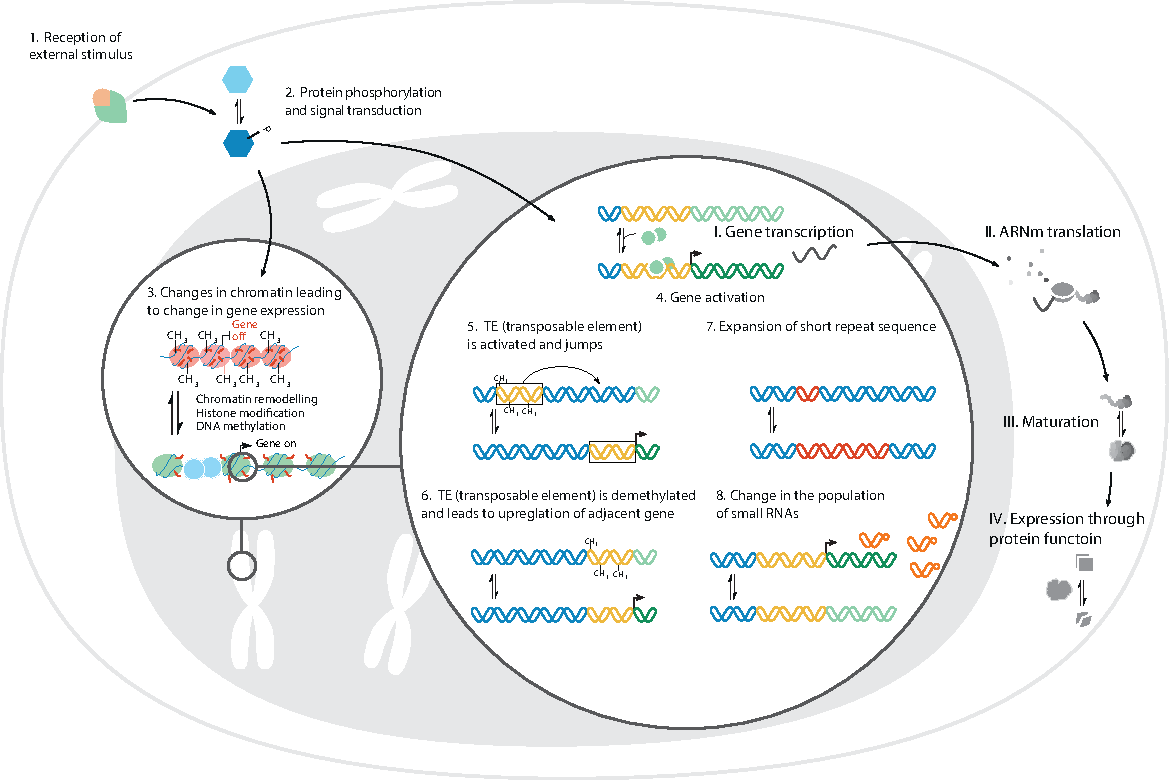
\includegraphics[width=1\linewidth]{./1_Introduction/graphics/molecular_basis.pdf}
  
%   \captionof{figure}{Caption}
   %\caption[Decomposition of plastic response]{Decomposition of phenotypic plasticity as a step between the genotype and the fitness. Phenotypic plasticity is the effect of environment on the link between genotype and phenotype. Plasticity can itself be decomposed in active plastic response that change the internal status of the individual (under genetic control) and passive response that result from inevitable effect of environment of the traits on the individual.}
%  \label{fig:plasticity_form}
%\end{figure}

The diversity of mechanisms and scales (both spatial and temporal) these processes can act inside of plant gives an idea of the diversity of strategies a plant can deploy to face changes of its environment. Considering this complexity, only a small fraction can be explored in such model as \model, but hopefully it will help make progress in our understanding of the role of these molecular mechanisms at the scale of the community.
\end{tcolorbox}
\end{fullwidth}






\paragraph{Forms of plasticity}
Phenotypic plasticity is the capacity of a species to produce individuals with the same genotype but different phenotypes. This difference in phenotype should be an active process, not the results of direct alteration of the phenotype by external factors without changes in internal functioning. This change in internal functioning process has the objective \sidenote{in the sense it has been selected because it provides this capacity} to match the phenotype with expected future conditions to maximise the individual fitness. The expression "expected future conditions" is key here, as it is this projection that drives the plasticity.
%Confusion, phenotypic plasticity is particular phenomenon, driven ...\\

\textit{Active plasticity is used for predominantly anticipatory, and often highly integrated, phenotypic changes in response to some environmental cue or signal, and reflect modifications of developmental pathways and regulatory genes.} Forsman - 2014\\


Passive plasticity, on the other hand, may stem from direct environmental influences on chemical, physiological and developmental processes, and is generally not considered anticipatory, but a mere consequence of the environment, such as stunted growth owing to low resource levels.\\


\begin{figure}
    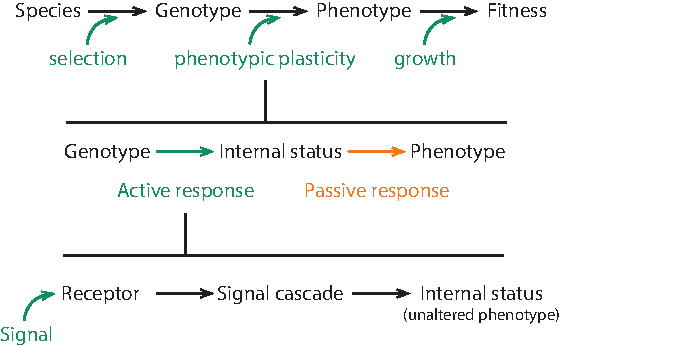
\includegraphics[width=1\linewidth]{./2_PP/Figures/Concepts/genotype_to_phenotype.pdf}
  \caption[Decomposition of plastic response]{Decomposition of phenotypic plasticity as a step between the genotype and the fitness. Phenotypic plasticity is the effect of environment on the link between genotype and phenotype. Plasticity can itself be decomposed in active plastic response that change the internal status of the individual (under genetic control) and passive response that result from inevitable effect of environment of the traits on the individual.}
  \label{fig:plasticity_form}
\end{figure}

%\paragraph{Biological process}
% The details of the molecular changes that occur in a plastic response ). 
Active and passive plastic response can be discriminated by the position of the control: internal for active plasticity, or external for passive response. In the case of active plastic response, the signal from environment must be integrated (from physical or chemical to information) then transferred to response organs. These organs respond to the integrated signal by changes in their expression levels (\textit{internal status} in figure \ref{fig:plasticity_form}) as summarised in figure \ref{fig:active_plasticity}.

Changes in phenotypes are controlled mainly by changes complex development processes. These processes involve numerous proetins and signaling pathways. Genes expression of proteins (transcription factors, enzymes, signalling proteins...) is controlled by specific mechanisms with various degrees of speed and duration (instantaneous regulation response, to inherited epigenetic adaptation). Some of these molecular processes are detailed in box \ref{box:molecular} in relationship with gene expression pathway (see also \cite{nicotra_plant_2010}).


\begin{marginfigure}
    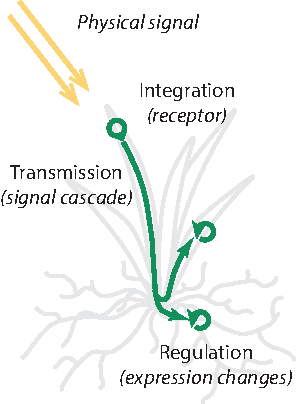
\includegraphics[width=1\linewidth]{./Figures/active_plasticity_m.pdf}
  \caption[Active plasticity]{Mechanism of active plasticity. Integration of a physical (or chemical) signal, transmission and regulation of phenotype through regulation of gene expression, or post-transcription regulations.}
  \label{fig:active_plasticity}
\end{marginfigure}

\textbf{Active phenotypic plasticity is an integrative process at the scale of the individual that aims for an improvement of plant fitness by the adjustment of its morphology according to environmental cues. It often relies on multiple regulation processes. Modelling the extend and the rules of such mechanism is not an easy task that might depend on the context and the framework used.}

%-----------------------------------------------------------------------------------------
\subsection{How to model phenotypic plasticity}

Plastic response can involve numerous genes interaction in networks of regulation pathways. The objective of an ecological model is not to reproduce this complexity, but the basic behaviours emerging from this biological complexity\sidenote{this biological complexity can be explained by the simplicity and limited number of basis biological units living organism are made of, and the emergence throuth simple mutation-selection operation. This complexity can be mimic by simpler and freer mathematical design.}. The basic components of the active plastic response are the perception of the external signal, its integration into meaningful information and the transformation into phenotype modification.

\paragraph{Reference and plastic traits}

%Modelling is compromise, a balance must be find between precision and consistency, between complexity and simplicity. This means that not all facets of a plant can be modelled, and simplifications must be adopted to have an efficient representation of a plant. The level o precision is defined by many aspects, but mostly the questions the modeller want to answer, and the main processes that drive the interrogated phenotmenon. In any case, the plant is represented by variables, that can be traits in ecology, that correspond to aggregates of a plant true characteristics. \cite{lucas_plant_2011} 
Every growth model is plastic. Every growth model predict different phenotypes for plants sharing the  same phenotype (often just defined by the species affiliation) growing in different condition. But most of this plasticity is passive, and it could be encompassed in this personnal definition of the notion of \textemph{growth function} (see figure \ref{fig:growth_function}). However, amoung vegetation models only some of them claim to include phenotypic plasticity \parencite{maire_plasticity_2013}, why so? What criterion can be used to distinguish active from passive plasticity in the context of plant modelling?

The use of information from environment to change the phenotype in order to have a better fitness is active plasticity. But in practice (in models)\parencite{maire_plasticity_2013}, often nothing really separates the two as plasticity is often modelled as a general mechanism shared by all species (but see \cite{jablonka_adaptive_1995} for discrete strategies in clonal plants) and local environmental variables are used to determine the phenotype of a plant in both cases. Only the justifications and the forms of the linking functions are different, and they may involve different traits. This idea is illustrated in figure \ref{fig:plastic_function}, where the phenotype is first defined by the genotype then controlled by the growth function as a function of current phenotype and environment (see figure \ref{fig:plastic_function}, left column). There is not differences between plasticity of two species, if two species have the same phenotype, then in similar environment they would express the same plastic response. I argue that plasticity, to be considered as an active process, should be under a genetic control (\textit{i.e.} species specific parameter). This means that, despite a shared rule and similar phenotype, the plastic would be different and would depend on a species specific parameter.


\begin{figure}
    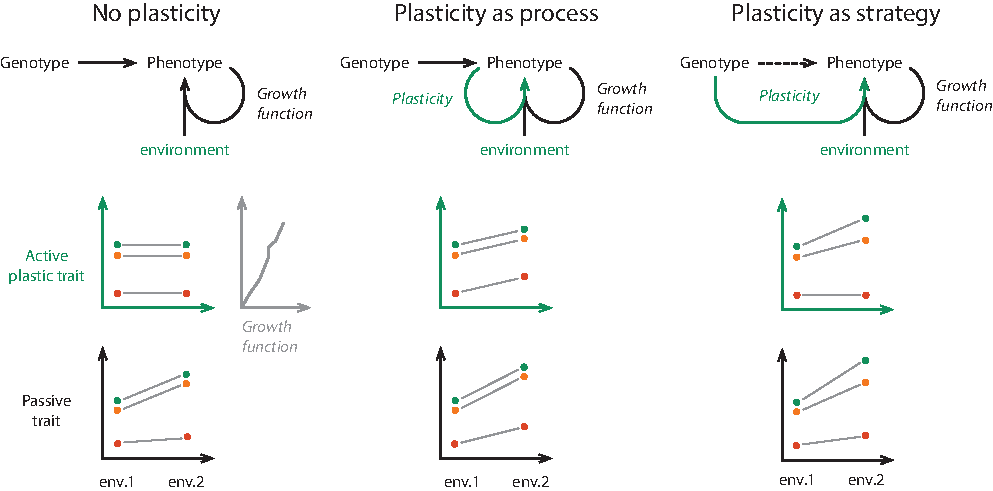
\includegraphics[width=1\linewidth]{./1_Introduction/graphics/plastic_function.pdf}
  \caption[Forms of plasticity in models]{Three forms of plasticity in models. }
  \label{fig:plastic_function}
\end{figure}

Moreover, no integration function, 

Two questions emerge from this: if growth function and plastic response are different (conceptually), how to determine each of these functions?
How the genetic control affect the phenotypic response? Or why would it be beneficial to have multiple rules - non discrete perspective on plasticity.

%However, the linking function used have different justifications and forms, and act of potentially different traits. In order to mimic active plasticity observed in nature the environmental variables should be integrated by plants, however this integration function is often ignored \cite{maire_plasticity_2013}. Therefore plasticity is mostly framed by the traits that are affected by the 


%One definition could be \textit{any variation of traits that alter plant functioning}, but that would not be enough as grazzing modification of  ... information to change traits ... hum OK, but mostly jsut a change in frame of reference. Still affect the niche.


%every model plastic, but mostly passive

we want active plasticity, what's distinguish plasticity types is not the frame of reference, but the strategy: it's a choice: determine by another trait that characterise the response.

what make it plastic: find the invariance. Laughlin? (what's invariance anyway)

\paragraph{Plasticity rules: a question of drivers}

defined by variable (ref plasticity is good in vairable) and limiting variables (resource, temp, perturbation) = drivers

functions: reaction norms \parencite{feller_mathematical_2015} thickness and light. Nice, but doesn't work with multiple drivers and composite traits

Or general rules : give a optimum phenotype. More deterministic approach. But optimum = general rule. Conceptually, if there is an optimum: why do something else ? Empirical studies: can be maladaptive, plasticity is a bet, and often ignore 

resources, but also risk (frost, grazing): alter cost and gains. Multi-process plasticity, with relative weights. see chapter \ref{part:synthesis}, section \ref{chapter:extension}.

%not often prediction, but just reaction norms: in that sense it is close to nature functioning, but ignore evolutionary mechanisms that selected these reaction norms (can take an more deterministic perspective on the matter).

Or perfect optimisation with perfect estimation of condition.





% to litteral 
%\textbf{Phenotypic plasticity requires two main components: (1) a projection of future conditions, (2) a link function between conditions and phenotype. The link function can have an additional parameter in the form of the current state of the individual, parameter that alters the form of the function.}
\textbf{}

% _______________________________________________________________________________________
\section{Toward an integrative framework of plant strategy and phenotypic plasticity}

Adaptive plasticity in models is often a layer on top of the species strategy, it acts more like a new mechanism, rather than a strategy within the already existing growth process. To interrogate the plasticity as a dimension of plant growth and an evolutionary process \parencite{bradshaw_evolutionary_1965} (see also work of Scheiner \parencite{scheiner_genetics_1989, scheiner_genetics_2002 ,scheiner_genetics_2012}), or better understand the cost and limits of plasticity \cite{dewitt_costs_1998, callahan_phenotypic_2008, auld_re-evaluating_2009}, or the effect of plasticity on coexistence and community dynamics \cite{hart_how_2016}, plant strategies and plasticity need to be blended together in an integrative framework.
%For models we talk about plastic models versus models that do not include plasticity. It makes sense to differentiate models based on the inclusion or not of plasticity, but if the plasticity is considered an important mechanism for the system, then we need to consider what's plastic and what's not. Traits 

\subsection{Plastic strategies}

Resource-use and allocation strategies have been related to environmental conditions in both empirical \parencite{wright_leaves_2002, ackerly_functional_2004, poorter_leaf_2006}, conceptual \parencite{grime_evidence_1977, westoby_leaf-height-seed_1998} and modelling\parencite{kleidon_global_2000, scheiter_impacts_2009, reineking_environmental_2006} studies. Moreover, functional traits show evidence of intra-spacific changes along environmental gradient \parencite{kichenin_contrasting_2013} and intra-specific economic spectrum \parencite{hu_novel_2015}, and constraints that shape main ecological trade-offs are certain to also constrain individual traits. Therefore, if strategies vary between and within species along environmental gradients, it makes sense to imagine that plasticity as changes in strategic traits. This goes beyond changes in spatial allocation\parencite{schapendonk_lingra_1998}, or parameters non identify as strategic traits \cite{lohier_explaining_2014, feller_mathematical_2015}. Considering strategic traits is not common practice because it blurs the limits between species that are not well identified by these traits any more\sidenote{especially when a relatively low number of species specific traits are considered}.

%Unlike the conception of plasticity in models \cite{ maire_plasticity_2013, lohier_explaining_2014}. Why? because blur the frontier between species, species specific traits are not thta specific anymore. But remember "species about trait than trait about species 
However, while this interpretation makes sense, the species and the individuals do not have the same constraints, and plasticity cannot be as large as intra-specific diversity as there are limitations to plastic development \parencite{dewitt_costs_1998, auld_re-evaluating_2009}. Moreover it seems that rules that drive plastic may not be the same as the ones that drive intra-specific genetic variations  and inter-specific differences\parencite{ryser_consequences_2000}, explaining contrasting response along gradient or between experimental drought treatment \parencite{kichenin_contrasting_2013, jung_intraspecific_2014}. This difference is probably more important for grass species than trees \parencite{franklin_modeling_2012} because of a lower scale difference between growth and selection processes.

%but attention, not also the same pattern  as certainly driven by different mechanisms 
\begin{quotation}
Phenotypic plasticity tends to maximize resource acquisition and growth rate in the short term, whereas the higher tissue-mass density and the longer leaf life-span of shade-tolerant species indicate reduced loss rates as a more advantageous species-specific adaptation to shade in the long term. - \cite{ryser_consequences_2000}
\end{quotation}



%strategies are adapted to conditions \cite{kleidon_global_2000, reineking_environmental_2006}, somehow it is logic that strategy should be adapted. Plasticity is in top, on some variables not specific. Is strategic, or plastic. Optimum concept: no need for specificity. 

\subsection{Plasticity as a strategy}

Most models consider plasticity in traits or carbon partitioning as a general behaviour that is present or absent for all considered species. While this discretisation of the phenomenon is not problematic, and rather informative for single plant or monoculture simulations \cite{maire_plasticity_2013}, it ignore the question of the adaptive value of plasticity and does not allow a continuous representation of plasticity.
%it ignores the evolutionary discussions around plasticity.

%true impact of plasticity 
%Not all species are plastic

%frame of reference: does not allow the interrogation of plasticity as a strategy. All plant share the same plasticity.

\paragraph{Cost and limits}

Intuitively phenotypic plasticity is a mechanism that increase fitness and has a positive adaptive value (increases the change to be selected). However multiple \textemph{costs} and limits have been identified, both biological \parencite{ dewitt_cost_1998, auld_re-evaluating_2009, callahan_phenotypic_2008} and ecological \parencite{dewitt_cost_1998, auld_re-evaluating_2009, scheiner_genetics_1989, scheiner_genetics_2002 ,scheiner_genetics_2012, van_kleunen_constraints_2005}, limiting the extend of plasticity observed in nature and differences between species (in grasslands see \cite{ryser_consequences_2000}).

...



\paragraph{Continuous plasticity}
These limitations, in addition to indicate the processes that should be included in dynamics models involving phenotypic plasticity, show that plasticity should be continuous. Indeed, costs of plasticity can increase with the amplitude of the plastic response and/or the complexity, therefore reducing the adaptive value of plasticity. Because non linearity can be expected between amplitude of plastic response and both fitness increase and cost, the adaptive value of plastic response can switch from positive to negative depending on its amplitude. Such behaviour would justify a non discrete plastic response (or variable sensitivity for polyphenism) to be captured in a model.
%
%Why is not always present: multiple arguements. auld dewitt murren
%requirements \parencite{van_kleunen_constraints_2005, valladares_ecological_2007}
%
%\cite{callahan_phenotypic_2008} cost of phenotype, and cost of plasticity


%
%It is not always present, and there are differences between species: plasticity selection must be integrated in models, as other traits
%
%ecological: maladaptive in different environment than what it was selected in \cite{dewitt_costs_1998} - cue reliability: \cite{valladares_ecological_2007}


\paragraph{From process to strategy}

As mentioned, ecological processes can favour or limit the selection of plasticity as any other trait. The idea of plasticity as a trait under genetic control is not new. Anthony Braddshaw was probably the first to defend this idea of genes controlling the variability of phenotypes. 
%\begin{quotation}
%Genes must exist not only to determine character means, but also to determine character response, which adds interesting complexity to our ideas about evolution. - \cite{bradshaw_unravelling_2006}
%\end{quotation}

But it is rarely implemented in individual or community growth model. This can be explained by the fact that plasticity is often seen as a process, rather than a strategy (see previous paragraph). In individual based model, plasticity as a process is often considered because of the relatively low number of species, and scientific question not focusing on ecological aspects. In models that consider the dynamics of diverse communities under drastic changes, integrating the plasticity as a strategy is crucial. This can be done by the use of species specific traits that control the amplitude and/or direction of the response (see more details in chapter \ref{part:model}). In population models, plasticity is often considered as a source of variation equivalent to intra-specific genetic variations and is modelled by a distribution function. \cite{dewitt_expanding_2016} proposes approaches with higher moments and environment dependent distribution to integrate plasticity into such models. In development models, bayesian model offer an unifying framework to combine inherited information and environmental cues \parencite{stamps_bayesian_2016}.
% To shift from plasticity as a process to plasticity as a strategy, the implementation of plasticity within model must change to integrate control over plastic response (amplitude and/or direction)\parencite{bradshaw_unravelling_2006}.
%bradshaw and dewitt, stamps?

%see paragraph \ref{subsection:bell-shape} 

%two sides on the relationship:
%- how pl affect evolution \cite{pfennig_phenotypic_2010} need to be investigated
This shift is also important, because if genes control plasticity, plasticity can also alter evolutionary process and therefore the response to climate change\cite{pfennig_phenotypic_2010, matesanz_global_2010, nicotra_plant_2010}.


%or community dynamics and properties: resistance and resilience. Plasticity of the 


%- how ecology and evolutionary processes allow and impact pl:
%evolution can impact plasticity as other traits


%rewrite this more positively with more content from the section ! 

\textbf{Plasticity is a complex matter, together a growth process that alter strategies and a strategy itself. New simulations tools for understanding community dynamics should try to both include multiple coexistence mechanisms and plant strategies, and focus on individual level mechanisms of competition, growth and survival. This can only be achieved in a constraint high dimensional strategy space based on physical and biological trade-offs. Individual level modelling allows the integration of multiple sources of intra-specific variability: genetic diversity and phenotypic plasticity. Phenotypic plasticity being driven by the perception of environment, it cannot be simply described by normal random distribution and should receive more attention. This focus is particularly important considering both the lack of understanding of this phenomena and the consequences for plant communities.}


\section{How phenotypic plasticity affect ecosystem properties and dynamics}

The difficulty to model phenotypic plasticity, more precisely to integrate multiple aspects of the complexity of phenotypic plasticity in the context of community dynamics, is limiting the current knowledge of the impact of this mechanism on community composition, properties and dynamics under global change. In this paragraph, I try to identify the mechanisms by which pheotypic plasticity impacts plant communities, and to determine if there are unresolved questions or paradoxes, or incomplete conclusions. The focus will be given to the main properties of the grassland communities: diversity, productivity and identity.

%The lack of representation of precise mechanism for pp - little idea how pl impact community, especially under changes in conditions (resistance, selection )


\subsection{Contrasting effect on diversity}

\textemph{Diversity} is a complex subject as discussed earlier in section \ref{chapter:coexistence}, resulting from various processes and measured by many indicators. Therefore, there are many ways the plasticity can affect diversity. Also the scope at which diversity is considered may change the effect of plasticity as the balance between may driving mechanism is shifted (see \cite{chalmandrier_communities_2015} for the importance of the scale on diversity). I will try to keep it simple and focus on measures of diversity at the scale of the community.
%reduce invasion and extinction because no local adaptation or pl \cite{morin_comparing_2009}
%Convergence ?
\paragraph{Species diversity}

Species diversity is driven on two levels, at large scales by abiotic conditions and filtering, and at lower scale, within this large potential niche defined by abiotic conditions, by competition and facilitation interactions. From this point of view, plasticity certainly increase the potential niche both along environmental conditions axis, but also along variation axis (species might be more or less sensitive to changes in conditions), therefore enlarging \textemph{niche} superposition \parencite{violle_return_2012}. This effect should in theory increase potential diversity as more species can potentially live in any given environment \parencite{lepik_high_2005, jung_intraspecific_2014}, but the effect of biotic interactions must be considered before drawing any conclusion of the effect of plasticity on realised diversity. The effect of plasticity on interactions is much harder to predict. According to \cite{adler_coexistence_2007} increase in niche difference and decrease in average fitness differences would increase stable coexistence.

The impact of plasticity mechanism on stabilizing effect is also hard to anticipate. It will likely be negative because established species may better fill any potential gap and prevent low density positive effect and therefore invasion \parencite{berg_trait_2010}. At the contrary, reduction of fitness difference due to plasticity could lead to stronger coexistence between species. Yet, the reduction of fitness differences is not guaranteed and in case of asymmetric gain (relative to strategies), plasticity could reduce realised diversity by increasing competitive exclusion.
There are here multiple effects (figure \ref{fig:effect_diversity} on species diversity that need to be disentangled. Recent review \parencite{turcotte_phenotypic_2016} of these effects show not consensus on the effect of phenotypic plasticity on stable coexistence.

\begin{figure}
    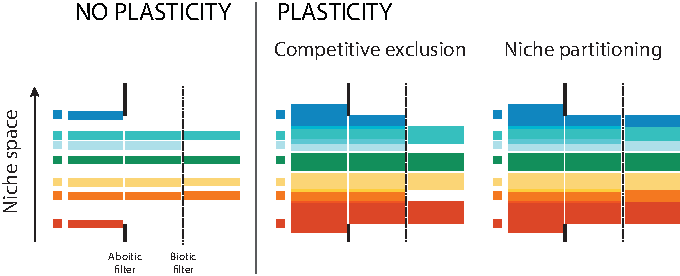
\includegraphics[width=1\linewidth]{./1_Introduction/graphics/filtering.pdf}
  \caption[Effect of plasticity of filters]{Phenotypic plasticity can affect filtering processes in diverse ways, making difficult the understanding of the role of plasticity in diversity maintenance.}
  \label{fig:plasticity_form}
\end{figure}

But plasticity responses not only depend on abiotic condition, but also on the neighbourhood that affects local environment \parencite{sultan_phenotypic_1995} at a fine scale. Because of platicity, these interactions can even shift from competition to facilitation \cite{callaway_phenotypic_2003}. A novel difficulty arises with the evidence that the identity of the competitor affect plastic response \parencite{callaway_phenotypic_2003, abakumova_plasticity_2016}, but it is likely that such interaction is related to traits and therefore impact on resource \parencite{callaway_phenotypic_2003}.

\paragraph{Functional diversity}

Species diversity often comes with functional diversity, however, phenotypic plasticity affect plant traits and is likely to affect functional diversity \parencite{albert_importance_2012}. Plasticity can lead to a convergence or a divergence of functional traits, decreasing or increasing functional diversity. In an experiment with legumes species \cite{roscher_contrasting_2015} observed these two phenomenons on different types of traits, between monoculture and mixture. The convergence of canopy filling and vertical growth traits suggests that competition stresses the different species on light competition, leading to a reduction of working strategies along these dimensions. Whereas, relatively, the other aspects of plant development are less constraint, or species experience diverse and contrasting conditions in mixture than in monoculture.



%directional changes
%Convergence vs non plastic trait diveristy.


\textbf{Phenotypic plasticity is expected to increase the potential niche of species and reduce the filtering effect of abiotic conditions. However, the effect on biotic interaction makes no consensus, and is likely to vary depending on the identity of the competitors, and the relative effect on trait differences. The balance between stabilizing niche differences and average fitness differences is crucial to determine the final impact on stable coexistence. The effects on functional diversity are also diverse but mainly depends on the plastic rules leading to convergence or divergence of traits.}
%But plasticity depends on neighbours: what does that change ?

%niche filling versus competitive exclusion: assymetric gain and coexistence theory.

\subsection{Productivity always improved?}

There is still debate on the effect of phenotypic plasticity of mechanisms driving species diversity, but is the question of the effect on productivity solved?

\paragraph{Stability}

Plasticity is a mechanism that emerges in situation where the plants can increase their fitness in response to environmental conditions. This increase in fitness is often due to higher resource use or resource foraging efficiency and therefore better growth rate (observed in models \parencite{maire_plasticity_2013} and empirical studies \parencite{ hamann_evidence_2016}). This leads to higher individual productivity. It is especially true when resources are varying and these variations can be anticipated  \cite{richter_phenotypic_2012}.

%Species able to deal with variations: stay relatively (more than without PP) when conditions doesn't match.

%pinus sylvestris gretter pl better in variable environment



\paragraph{Costs and limits}

However, has mentioned earlier, plasticity comes with inherent costs, related to the biological machinery needed to sense and process the signals and alter the phenotype. This costs, if the plant does not take advantage of the plasticity (no variability, in its niche) to increase (or maintain) growth rate will impact the productivity.

The unreliability of environmental cues is a limit of plasticity, and it can lead to maladaptive changes in phenotypes, but this is a marginal behaviour, and maladaptive plasticity is expected to be eliminated by evolutionary process in fairly constant conditions. However, in the context of climate change, the reliability of these cues may decrease and leads to maladaptive responses. 

If unnecessary costs and unreliable cues can impact overall plant efficiency, adaptive plasticity can also hurt productivity while increasing fitness. Indeed, as evolutionary models and game theory predict, competition can lead to lower efficiency than optimum arrangement. Competition leading to lower resource availability, plastic species may have an aggressive plastic response leading to stronger competitor but with less effective resource use.

%Competition behaviour may lead to suboptimum phenotypes.

\paragraph{Diversity and productivity}

Biodiversity - productivity
%
%Effects on
%
%Maintain different species: may change the productivity pattern. better at low prod, lower prod by introducing less productive species.


\subsection{Community identity shift}

The third main property of grassland communities is the \textemph{identity} of the dominant species (or average species if CWMs are considered). Phenotypic plasticity can impact community identity in two ways: (1) by shifting the identity of present species, (2) by altering the output of filtering processes in favour of different traits.

The first effect makes sense only in the context of a change in condition. Drought experiment in mountain grasslands show intra-specific shift toward higher LDMC and lower SLA \parencite{jung_intraspecific_2014}. Other empirical studies show uncoupled response between above- and below-ground organs, shifting the strategy of the species \parencite{freschett_plasticity_2014}.

A modelling experiment show that the phenotypic plasticity is required to correctly model the dominance pattern along cutting frequency gradient \parencite{maire_plasticity_2013}, illustrating the second effect. 

%selection of more or less resistant/digest/etc... species

%\textbf{Plasticity affect community identity by two independent mechanisms that might have contrasting outcomes. Both should be considered, therefore models should include both plastic resposne and population dynamics processes.}


\begin{figure}
    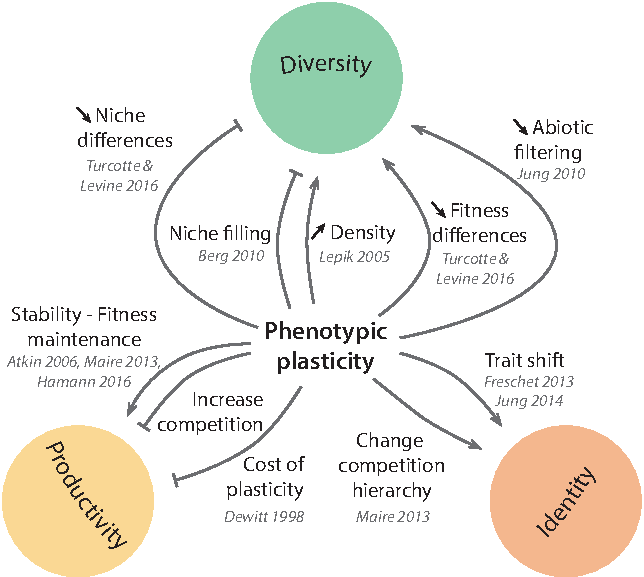
\includegraphics{./1_Introduction/graphics/effect_plasticity.pdf}
  \caption[Phenotypic plasticity effect on community properties]{Effect of phenotypic plasticity on the three main community properties. Phenotypic plasticity can impact these properties through multiple processes that may have contrasting effects. To determine the overall effect of plasticity on community response to changes in drivers (climate and land-use) we need to integrate all these effects.}
  \label{fig:plasticity-effect}
\end{figure}

\subsection{Phenotypic plasticity effect on individuals and communities}

% section/chapter concluesion
%\paragraph{Contrasting effects}
%
%\paragraph{Interacting mechanisms}

% try to extract guidelines from the review of litterature.


% begining on guide lines. Probably need high level of modification
\textbf{Plasticity is a complex matter, together a growth process that alter strategies and a strategy itself. New simulations tools for understanding community dynamics should try to both include multiple coexistence mechanisms and plant strategies, and focus on individual level mechanisms of competition, growth and survival. This can only be achieved in a constraint high dimensional strategy space based on physical and biological trade-offs. Individual level modelling allows the integration of multiple sources of intra-specific variability: genetic diversity and phenotypic plasticity. Phenotypic plasticity being driven by the perception of environment, it cannot be simply described by normal random distribution and should receive more attention. This focus is particularly important considering both the lack of understanding of this phenomena and the consequences for plant communities.  }


% _______________________________________________________________________________________

%\chapter{A new interface to explore} %##################################################
%
%
%\subsection{Vegetation community}
%
%\subsection{Basis of coexistence}
%
%\paragraph{Niche theory}
%
%%_______________________________________________________________________________________
%\section{On strategy and traits}
%
%\subsection{From species to traits}
%
%\subsection{Traits and strategy space}
%
%%_______________________________________________________________________________________
%\section{What is phenotypic plasticity}
%
%\subsection{The importance of intra-specific variability}
%
%\paragraph{Mean traits are not enough}
%
%\paragraph{The source of the variation}
%
%\paragraph{Different impacts on mechanisms}
%
%\subsection{Phenotipyc plasticity: a form of intraspecific variation}
%
%\paragraph{From genotype to phenotype}
%
%\paragraph{New references}
%
%\subsection{Extent of plasticity}
%
%\paragraph{Advantage}
%
%\paragraph{Costs}
%
%\paragraph{Limits}
%
%%_______________________________________________________________________________________
%\chapter{Strategy space and community modelling} %####################################
%
%
%
%%_______________________________________________________________________________________
%\chapter{Phenotypic plasticity and trait variations}   %##############################
%
%%_______________________________________________________________________________________
%\chapter{Community dynamics and the role of intra-specific variability} %#############
%

%
%\chapter{On coexistence and diversity}
%
%\section{Diversity and coexistence mechanisms}\label{sec:coexistence}
%
%Diversity of natural systems have long been a subject of admiration but also a mystery to the scientific community. The extraordinary multitude of species and individuals living at the same time, in the same space, is hard to reproduce and to explain. This is particularly true in plankton communities where the resources are limited to few nutrients (nitrate, phosphates) and light. Early coexistence theories, like the competitive exclusion principle that predicts that the number of coexisting species at equilibrium can at most be equal to the number of limiting resources, fail to explain such variety. This gap between empirical observation of high diversity in different systems and at different scales, and the lack of theoretical explanation was called the \textit{plankton paradox}. This paradox has now received multiples answers \textbf{NEED REFS}\sidenote{discussed in later in subsection \ref{ssec:div-mech}.}, but diversity and coexistence mechanisms are still investigated \parencite{falster_plant:_2016}. This illustrates our will to understand these mechanisms, but why are we still struggling with questions that animated ecologist decades ago? and why are we still interested by these questions? It is hard to answer the first interrogation, but the diversity of the interactions within such systems and the diversity and variability of external drivers shaping them are the main factors. That also explains partly the second question, and why scientists explore the genetic diversity of gut bacteria, or the phylogenetic diversity of phytoplankton in lakes, or the diversity of plants species from tropical forest of Brazil to snowy slopes of Alps. But besides the curiosity of scientists, studying the machinery behind the functioning the natural communities is essential if we want to understand and predict how they can evolve under the pressure of changing drivers, and how they can be managed. The following paragraphs attempt to explain the value of diversity, and so why we have to predict and manage it at best, and where is our current understanding of underlying mechanisms.\\
%
%\indent I may have been a bit far. Recentrate around mountain grasslands
%
%\subsection{Effects of diversity}
%Conservation\\
%productivity\\
%resistance ?\\
%Ecosystem services and complementarity\\
%
%\section{Mechanisms for coexistence, trade-offs and strategy spaces}\label{ssec:div-mech}
%main theories: niche, neutral, individual based. -> scale and dimension dependant.\\
%chesson \parencite{chesson_mechanisms_2000}\\
%Spatial and temporal variability\\
%trade-off, strategy space, and variability.\\
%in the end it's rarely direct interaction but capacity to respond to stress and interect interaction through resource pools.
%
%
%\section{About trade-off}
%chemical physical trade-off vs ecological trade-off.
%
%
%\section{Strategy spaces}
%
%
%\chapter{Intra-specific diversity and plasticity}
%\label{sec:intraspe}
%
%
%\section{Community dynamics: from individuals to group dynamics}
%\textbf{Need to  highligth how community dynamics emerge from individual response and interactions.}
%
%\section{Intra-specific variability}
%frame of reference: deep traits vs shallow traits. definition of functional trait.\\
%source of intra specific variability: genetic vs ontogeny vs plasticity (epigen) \\
%effect on niche and interactions: effect on coexistence\\
%-> plasticity a special form of ISV
%
%\section{Understanding phenotypic plasticity}
%
%%what is it, how it works or doesn't
%
%Bradshaw, sultan
%
%adaptive intraspecific variation\\
%cost and limits van kleunen, Dewitt and sultan \\
%effect on coexistence and community\\
%
%\begin{fullwidth}
%\begin{tcolorbox}[title=Molecular basis of phenotypic plasticity] %Toutes les options définies dans le préambule peuvent être définies aussi ici. J’ai juste gardé la possibilité de changer le titre de la box dans ma thèse
%Phenotypic plasticity lies both in the perception of external conditions through sensor organ and signaling pathways (auxin pathway, root stones for gravity ...), and the integration of this information to alter the development plan. This integration must be coordinated at the scale of the plant according to rules or objectives, question partly explore in this work, but ultimately is applied at the cell levels.\\
%\indent Because of the complexity and our partial understanding of these mechanisms, we will not attempt to model them. However I hope that this little overview of molecular mechanisms at the scale of the cell will give the reader an idea of the processes behind the abstract concepts used in this manuscript.\\
%
%BLABLABLA and figure\\
%
%The diversity of mechanisms and scales (both spatial and temporal) these processes can act inside of plant gives an idea of the diversity of strategies a plant can deploy to face changes of its environment. Considering this complexity, only a small fraction can be explored in such model as \model, but hopefully it will help make progress in our understanding of the role of these molecular mechanisms at the scale of the community.
%\end{tcolorbox}
%\end{fullwidth}
%
%\chapter{Niche, competition and coexistence with intraspecific variability}
%
%\textbf{Go beyond bell-shaped niche and symmetric competition. Trait analysis and mechanistic approaches defend more complex theories and complexity. Need tools integrating flexibility and complexity. Science is measure the relative balance between different effects/mehcanisms. Cannot be simplified to one simple mechanisms, but look when (what conditions) is more important than the other, how one is closer to real system, what properties this has.}
% 
%
%\chapter{Existing modelling approaches}
%\section{Global change effect on vegetation community}
%
%Message: modelling coexistence is a challenge because 1) do not know/understand all mechanisms, 2) challenging to incorporate enough mechanisms, 3) costly computation and data wise. -> need for more generic and complete (multiple mechanisms approaches.\\
%
%DGVMs\\
%IBMs
%
%
%\section{Modelling vegetation - traits and strategies}
%traits \& strategies\\
%existing models: a gap to fill\\
%coexistence processes
%
%\section{Modelling phenotypic plasticity}
%Reaction norms\\
%Source sink models\\
%Functional-Structural plant models FSPMs ? vos 2009\\
%Functional equilibrium. Somehow similar to the source sink in its philosophy, it allows optimisation of phenotype for multiple resources. \\


%
%
%%_________________________________________________________________________________
%\chapter{Mountain grasslands}
%\fwnewthought{Mountain grasslands have an unique beauty drawn by the diversity of flowers colours, the strong contrast between the luxurious green vegetation and the roughness of the naked rocks, and the feeling that living in such places, at the edge of living conditions, is a fight worth fighting. I could illustrate this beauty with thousands pictures and words, and it would certainly convince you that these ecosystems worth spending time studying them to better understand and protect them. I could also describe their role in the economy of alpine regions, currently subject of great modification, and greater to come. But you would not see these rich systems as I see them: as an intricate network of interaction living creatures, with their own characteristics, strategy and experience, forming a dynamic system... Capturing this beauty is one challenge of this modelling PhD.\\
%I must now give you an overview on the mountain grasslands}
%
%
%%\section{Photograph of mountain grasslands}
%The idea is to go from context, to services to ecology. At the entd of this part, it is obvious that ecosystem services can be derived from traits and that we need tools for prediction of MG dynamics.
%
%\section{Geography, climate and managements: les drivers}
%
%
%\section{Mountain grasslands under climate change}
%
%\section{Mountain grasslands, source of services}
%
%\section{Let's talk about traits} % might not be at the right place here
%response trait and effect traits (?) <- you need to talk about this to better introduce the shift from there to a deep/low level traits to composite traits (SLA if related to a certain resource use strategy, is also a composite trait (Nitrogen, light and water all affect the SLA value). View such traits as mono dimensional is dangerous as it simplify a lot (and I might have fallen within this trap). Having low level traits that define the overall strategy (and not how to achieve it) should help to have a more systemic view (good term here ? view of the system with all its parts) and better understand the rules that drive the development. But they also imply the need for new mechanisms to link such traits and strategies to actual, measurable traits that define the phenotype as we see it (at the level of interaction or services profides). \\
%Opportunity to emphasis the fact (a simple scheme should help here) that apparent traits are usefull (and measurable) to define the current effect on the environment (and so interactions between plants) and on provided services, but they are difficult to use to predict the dynamic of individuals and communities (precisely because they are changing and composit traits that respond to the environment).
%
%
%
%%_________________________________________________________________________________
%\chapter{Modelling ecological systems}
%The message here should be that: we know how to model vegetation systems, but we need finer resolution (from species and com, to traits, to individual responses) and bigger (higher number of species) scale -> generic framework and individual response.\\
%Based on two particular similar models: taubert, and Lohier.
%
%\section{Models as understanding and testing tools}
%
%\begin{quote}
%"Physicien de la biologie"
%\end{quote}
%Justify the modelling approach - what's a model ? simplification of reality\\
%Long subject refer to models in ecosystem sciences. Different classes of model, and different objectives. Mechanistic models: understanding and testing hypothesis.\\
%Model as understanding tools: how does modelling help us understanding the system we are modelling.\\
%The need for mechanistic model and emergent properties of models. Process-based models vs statistical model (what happen outside the data (example of flickering tails of regression models), similar to bayesian approach, the model is constrained by our understanding of processes.) \\
%mechanistic models: risks of lack of mechanisms, complex calibration, lot of parameters. Statistical model have the advantage of parcymony: minimum number of parameters to reproduce a pattern.
%
%\section{Modelling plant communities}
%
%\subsection{Different levels of modelling: from communities to individuals}
%community approaches, CWM to importance of individuals.\\
%
%
%\subsection{Processes}
%\paragraph{Test pragraph title - now what happen if it lays on multiples lines} This is a paragraphe \lipsum[2]
%
%\marginnote{\textbf{some notes}}
%\marginnote{\lipsum[1]}
%\sidenote{a short sidenote}
%
%\subsection{Agent-based models}
%
%Review of existing models (grasslands and forest)\\
%Comparison of two existing models\\
%How to build aroung/from that.\\
%
%
%\section{Modelling coexistence}
%Message: modelling coexistence is a challenge because 1) do not know/understand all mechanisms, 2) challenging to incorporate enough mechanisms, 3) costly computation and data wise. -> need for more generic and complete (multiple mechanisms approaches.
%
%\subsection{What is diversity and why model it?}
%
%On why model coxistence: better understanding of mechanisms, tool to evaluate and predict changes in coexistence.
%
%\begin{figure}
%\includegraphics[scale=1]{./1_Introduction/graphics/plankton.jpg}
%\end{figure}
%
%\subsection{The concept of niche}
%
%
%\subsection{Coexistence mechanisms}
%
%\section{Breaking the resolution-specificity trade-off}
%use of generic species\\
%still a trade-off with scale.
%
%%_________________________________________________________________________________
%\chapter{Phenotypic plasticity of organisms}
%Message here ?
%
%\section{Stability and plasticity}
%
%\section{Costs and limits of plasticity}
%
%\section{Plasticity and coexistence}
%
%
%%__________________________________________________________________________________
%\chapter*{Scientific questions}
%How to model vegetation system with higher resolution at bigger scale?\\
%How does plasticity work in plants?\\
%Effect of plasticity of plant interactions (and coexistence)?\\
%Effect of plasticity on resistance/resilience to climatic events?\\
%Effect of this mechanism on overall services provision?








%\section{What's a trade-of}

%\lipsum[1]
%
%\begin{figure}
%\begin{tikzpicture}
%\begin{axis}[plot]
%\addplot[teal,
%xtick=data]
%coordinates {(0, 0) (1, 1) (2, 2)};
%\end{axis}
%\end{tikzpicture}
%\caption{Test figure to setup pgfplots in Tufte environment}
%\end{figure}
%
%\lipsum[1-3]
%
%\begin{marginfigure}
%\begin{tikzpicture}
%\begin{axis}[marginplot]
%\addplot[teal] coordinates {(0, 0) (1, 1) (2, 2)};
%\end{axis}
%\end{tikzpicture}
%\caption{Test figure to setup pgfplots in Tufte environment}
%\end{marginfigure}

\end{document}